\section{Tutorial B2}

\begin{problem}
    \begin{center}\tikzsetnextfilename{235}
        \begin{tikzpicture}[trim axis left, trim axis right]
            \begin{axis}[
                samples = 101,
                axis y line=middle,
                axis x line=middle,
                xtick = \empty,
                ytick = \empty,
                xlabel = {$x$},
                ylabel = {$y$},
                legend cell align={left},
                legend pos=outer north east,
                after end axis/.code={
                    \path (axis cs:0,0) 
                        node [anchor=north east] {$O$};
                    }
                ]
                \addplot[plotRed, domain=-1:1] {-x+1};

                \addplot[plotRed, domain=1:2] {x-1};

                \addplot[plotRed, domain=2:5] {-x+3};
    
                \addlegendentry{$y = f(x)$};

                \fill (0,1) circle[radius = 2.5pt] node[anchor=west] {$A(0, 1)$};

                \fill (1, 0) circle[radius = 2.5pt] node[anchor=north] {$B(1, 0)$};

                \fill (2,1) circle[radius = 2.5pt] node[anchor=south] {$C(2, 1)$};

                \fill (3,0) circle[radius = 2.5pt] node[anchor=south west] {$D(3, 0)$};
            \end{axis}
        \end{tikzpicture}
    \end{center}

    The graph of $y = f(x)$ is shown here. The points $A$, $B$, $C$ and $D$ have coordinates $(0, 1)$, $(1, 0)$, $(2, 1)$ and $(3, 0)$ respectively. Sketch, separately, the graphs of 

    \begin{enumerate}
        \item $y=f(2x)$
        \item $y=f(x+3)$
        \item $y = 1 - f(x)$
        \item $y = 3f\bp{\frac{x}2 - 1}$
    \end{enumerate}
    stating, in each case, the coordinates of the points corresponding to $A$, $B$, $C$ and $D$.
\end{problem}
\begin{solution}
    \begin{ppart}
        \begin{center}\tikzsetnextfilename{236}
            \begin{tikzpicture}[trim axis left, trim axis right]
                \begin{axis}[
                    samples = 101,
                    axis y line=middle,
                    axis x line=middle,
                    xtick = \empty,
                    ytick = \empty,
                    xlabel = {$x$},
                    ylabel = {$y$},
                    legend cell align={left},
                    legend pos=outer north east,
                    after end axis/.code={
                        \path (axis cs:0,0) 
                            node [anchor=north east] {$O$};
                        }
                    ]
                    \addplot[plotRed, domain=-1:1] {-x+1};

                    \addplot[plotRed, domain=1:2] {x-1};

                    \addplot[plotRed, domain=2:5] {-x+3};
        
                    \addlegendentry{$y = f(2x)$};

                    \fill (0,1) circle[radius = 2.5pt] node[anchor=west] {$A(0, 1)$};

                    \fill (1, 0) circle[radius = 2.5pt] node[anchor=north] {$B\bp{\frac12, 0}$};

                    \fill (2,1) circle[radius = 2.5pt] node[anchor=south] {$C(1, 1)$};

                    \fill (3,0) circle[radius = 2.5pt] node[anchor=south west] {$D\bp{\frac32, 0}$};
                \end{axis}
            \end{tikzpicture}
        \end{center}
    \end{ppart}
    \clearpage
    \begin{ppart}
        \begin{center}\tikzsetnextfilename{237}
            \begin{tikzpicture}[trim axis left, trim axis right]
                \begin{axis}[
                    samples = 101,
                    axis y line=middle,
                    axis x line=middle,
                    xtick = \empty,
                    ytick = \empty,
                    xlabel = {$x$},
                    ylabel = {$y$},
                    legend cell align={left},
                    legend pos=outer north east,
                    after end axis/.code={
                        \path (axis cs:0,0) 
                            node [anchor=north east] {$O$};
                        }
                    ]
                    \addplot[plotRed, domain=-5:-2] {-x-2};

                    \addplot[plotRed, domain=-2:-1] {x+2};

                    \addplot[plotRed, domain=-1:2] {-x};
        
                    \addlegendentry{$y = f(x+3)$};

                    \fill (-3,1) circle[radius = 2.5pt] node[anchor=north east] {$A(-3, 1)$};

                    \fill (-2, 0) circle[radius = 2.5pt] node[anchor=north] {$B(-2, 0)$};

                    \fill (-1,1) circle[radius = 2.5pt] node[anchor=south] {$C(-1, 1)$};

                    \fill (0,0) circle[radius = 2.5pt] node[anchor=south west] {$D(0, 0)$};
                \end{axis}
            \end{tikzpicture}
        \end{center}
    \end{ppart}
    \begin{ppart}
        \begin{center}\tikzsetnextfilename{238}
            \begin{tikzpicture}[trim axis left, trim axis right]
                \begin{axis}[
                    samples = 101,
                    axis y line=middle,
                    axis x line=middle,
                    xtick = \empty,
                    ytick = \empty,
                    xlabel = {$x$},
                    ylabel = {$y$},
                    legend cell align={left},
                    legend pos=outer north east,
                    after end axis/.code={
                        \path (axis cs:0,0) 
                            node [anchor=south east] {$O$};
                        }
                    ]
                    \addplot[plotRed, domain=-1:1] {x};

                    \addplot[plotRed, domain=1:2] {-x+2};

                    \addplot[plotRed, domain=2:5] {x-2};
        
                    \addlegendentry{$y = 1-f(x)$};

                    \fill (0, 0) circle[radius = 2.5pt] node[anchor=north west] {$A(0, 0)$};

                    \fill (1, 1) circle[radius = 2.5pt] node[anchor=south] {$B(1, 1)$};

                    \fill (2, 0) circle[radius = 2.5pt] node[anchor=north] {$C(2, 0)$};

                    \fill (3, 1) circle[radius = 2.5pt] node[anchor=west] {$D(3, 1)$};
                \end{axis}
            \end{tikzpicture}
        \end{center}
    \end{ppart}
    \begin{ppart}
        \begin{center}\tikzsetnextfilename{239}
            \begin{tikzpicture}[trim axis left, trim axis right]
                \begin{axis}[
                    samples = 101,
                    axis y line=middle,
                    axis x line=middle,
                    xtick = \empty,
                    ytick = \empty,
                    xlabel = {$x$},
                    ylabel = {$y$},
                    ymin=-2,
                    xmax=10,
                    legend cell align={left},
                    legend pos=outer north east,
                    after end axis/.code={
                        \path (axis cs:0,0) 
                            node [anchor=east] {$O$};
                        }
                    ]
                    \addplot[plotRed, domain=0:4] {-3/2 * x + 6};

                    \addplot[plotRed, domain=4:6] {3/2 * x - 6};

                    \addplot[plotRed, domain=6:8] {-3/2 * x+12};
        
                    \addlegendentry{$y = 3f\bp{\frac{x}{2} - 1}$};

                    \fill (2, 3) circle[radius = 2.5pt] node[anchor=west] {$A(2, 3)$};

                    \fill (4, 0) circle[radius = 2.5pt] node[anchor=north] {$B(4, 0)$};

                    \fill (6, 3) circle[radius = 2.5pt] node[anchor=south] {$C(6, 3)$};

                    \fill (8,0) circle[radius = 2.5pt] node[anchor=north] {$D(8, 0)$};
                \end{axis}
            \end{tikzpicture}
        \end{center}
    \end{ppart}
\end{solution}

\begin{problem}
    Sketch, on a single clear diagram, the graphs of 

    \begin{enumerate}
        \item $y = x^2$
        \item $y = (x+a)^2$
        \item $y = b(x+a)^2$
        \item $y = b(x+a)^2 + c$
    \end{enumerate}

    Assume constants $a > 0$, $c > 0$ and $b > 1$.
\end{problem}
\begin{solution}
    \begin{center}\tikzsetnextfilename{240}
        \begin{tikzpicture}[trim axis left, trim axis right]
            \begin{axis}[
                domain=-5:4,
                samples = 101,
                axis y line=middle,
                axis x line=middle,
                xtick = {-2},
                xticklabels = {$-a$},
                ytick = {4, 8, 11},
                yticklabels = {$a^2$, $ba^2$, $ba^2 + c$},
                xlabel = {$x$},
                ylabel = {$y$},
                ymin=-2,
                xmax=4,
                ymax=13,
                legend cell align={left},
                legend pos=outer north east,
                after end axis/.code={
                    \path (axis cs:0,0) 
                        node [anchor=north east] {$O$};
                    }
                ]
                \addplot[plotRed] {x^2};
    
                \addlegendentry{$y =x^2$};

                \addplot[plotBlue] {(x+2)^2};
    
                \addlegendentry{$y =(x+a)^2$};

                \addplot[plotGreen] {2 * (x + 2)^2};
    
                \addlegendentry{$y = b(x+a)^2$};

                \addplot[plotBlack] {2 * (x + 2)^2 + 3};
    
                \addlegendentry{$y = b(x+a)^2 + c$};

                \fill (-2, 3) circle[radius=2.5 pt] node[anchor=north, fill=white, opacity = 0.6, text opacity=1] {$(c, -a)$};
            \end{axis}
        \end{tikzpicture}
    \end{center}
\end{solution}

\begin{problem}
    The graph below has equation $y = f(x)$. It has asymptotes $y = 1$ and $y = 0$, a maximum point at $D(1, 2)$, a minimum point at $A(-2, -1)$, cuts the $x$-axis at $B(-1. 0)$ and cuts the $y$-axis at $C(0, 1)$.

    \begin{center}\tikzsetnextfilename{241}
        \begin{tikzpicture}[trim axis left, trim axis right]
            \begin{axis}[
                domain=-5:4,
                samples = 101,
                axis y line=middle,
                axis x line=middle,
                xtick = \empty,
                ytick = \empty,
                xlabel = {$x$},
                ylabel = {$y$},
                ymin=-2,
                ymax=3.5,
                legend cell align={left},
                legend pos=outer north east,
                after end axis/.code={
                    \path (axis cs:0,0) 
                        node [anchor=north east] {$O$};
                    }
                ]
                \addplot[plotRed, domain=-5:-2] {(0.5 * e^(0.5)) * x * e^(-1/8 * x^2)};

                \addplot[plotRed, domain=-2:1] {x+1};

                \addplot[plotRed, domain=1:4] {(e^(0.5) * x * e^(-0.5 * x^2)) + 1};

                \addlegendentry{$y = f(x)$};

                \fill (-2, -1) circle[radius=2.5 pt] node[anchor=north] {$A(-2, -1)$};

                \fill (-1, 0) circle[radius=2.5 pt] node[anchor=south east] {$B(-1, 0)$};

                \fill (0, 1) circle[radius=2.5 pt] node[anchor=south east] {$C(0, 1)$};

                \fill (1, 2) circle[radius=2.5 pt] node[anchor=south] {$D(1, 2)$};

                \draw[dotted, thick] (4, 1) -- (-5, 1) node[anchor=south west] {$y=1$};
            \end{axis}
        \end{tikzpicture}
    \end{center}

    Sketch on separate diagrams the graphs of the following curves, labelling each curve clearly, indicating the horizontal asymptotes and showing the coordinates of the points corresponding to the points $A$, $B$, $C$ and $D$.
    
    \begin{enumerate}
        \item $y = f(x+1)$
        \item $y = f\bp{\frac{x}2}$
        \item $y = 2f(x) - 2$
    \end{enumerate}

    Find the number of solutions to the equation $f(x) = af(x)$ where $a \geq 2$.
\end{problem}
\clearpage
\begin{solution}
    \begin{ppart}
        \begin{center}\tikzsetnextfilename{242}
            \begin{tikzpicture}[trim axis left, trim axis right]
                \begin{axis}[
                    domain=-6:3,
                    samples = 101,
                    axis y line=middle,
                    axis x line=middle,
                    xtick = \empty,
                    ytick = \empty,
                    xlabel = {$x$},
                    ylabel = {$y$},
                    ymin=-2,
                    ymax=3.5,
                    legend cell align={left},
                    legend pos=outer north east,
                    after end axis/.code={
                        \path (axis cs:0,0) 
                            node [anchor=north east] {$O$};
                        }
                    ]
                    \addplot[plotRed, domain=-6:-3] {(0.5 * e^(0.5)) * (x+1) * e^(-1/8 * (x+1)^2)};

                    \addplot[plotRed, domain=-3:0] {(x+1)+1};

                    \addplot[plotRed, domain=0:3] {(e^(0.5) * (x+1) * e^(-0.5 * (x+1)^2)) + 1};

                    \addlegendentry{$y = f(x+1)$};

                    \fill (-3, -1) circle[radius=2.5 pt] node[anchor=north] {$A(-3, -1)$};

                    \fill (-2, 0) circle[radius=2.5 pt] node[anchor=south east] {$B(-2, 0)$};

                    \fill (-1, 1) circle[radius=2.5 pt] node[anchor=south east] {$C(-1, 1)$};

                    \fill (0, 2) circle[radius=2.5 pt] node[anchor=south west] {$D(0, 2)$};

                    \draw[dotted, thick] (3, 1) -- (-6, 1) node[anchor=south west] {$y=1$};
                \end{axis}
            \end{tikzpicture}
        \end{center}
    \end{ppart}
    \begin{ppart}
        \begin{center}\tikzsetnextfilename{243}
            \begin{tikzpicture}[trim axis left, trim axis right]
                \begin{axis}[
                    domain=-10:8,
                    samples = 101,
                    axis y line=middle,
                    axis x line=middle,
                    xtick = \empty,
                    ytick = \empty,
                    xlabel = {$x$},
                    ylabel = {$y$},
                    ymin=-2,
                    ymax=3.5,
                    legend cell align={left},
                    legend pos=outer north east,
                    after end axis/.code={
                        \path (axis cs:0,0) 
                            node [anchor=north east] {$O$};
                        }
                    ]
                    \addplot[plotRed, domain=-10:-4] {(0.5 * e^(0.5)) * (x/2) * e^(-1/8 * (x/2)^2)};

                    \addplot[plotRed, domain=-4:2] {(x/2)+1};

                    \addplot[plotRed, domain=2:8] {(e^(0.5) * (x/2) * e^(-0.5 * (x/2)^2)) + 1};

                    \addlegendentry{$y = f\bp{\frac{x}2}$};

                    \fill (-4, -1) circle[radius=2.5 pt] node[anchor=north] {$A(-4, -1)$};

                    \fill (-2, 0) circle[radius=2.5 pt] node[anchor=south east] {$B(-2, 0)$};

                    \fill (0, 1) circle[radius=2.5 pt] node[anchor=south east] {$C(0, 1)$};

                    \fill (2, 2) circle[radius=2.5 pt] node[anchor=south] {$D(2, 2)$};

                    \draw[dotted, thick] (8, 1) -- (-10, 1) node[anchor=south west] {$y=1$};
                \end{axis}
            \end{tikzpicture}
        \end{center}
    \end{ppart}
    \begin{ppart}
        \begin{center}\tikzsetnextfilename{244}
            \begin{tikzpicture}[trim axis left, trim axis right]
                \begin{axis}[
                    domain=-5:4,
                    samples = 101,
                    axis y line=middle,
                    axis x line=middle,
                    xtick = \empty,
                    ytick = \empty,
                    xlabel = {$x$},
                    ylabel = {$y$},
                    ymin=-6,
                    ymax=5,
                    legend cell align={left},
                    legend pos=outer north east,
                    after end axis/.code={
                        \path (axis cs:0,0) 
                            node [anchor=north west] {$O$};
                        }
                    ]
                    \addplot[plotRed, domain=-5:-2] {2*((0.5 * e^(0.5)) * x * e^(-1/8 * x^2)) - 2};

                    \addplot[plotRed, domain=-2:1] {2*(x+1) - 2};

                    \addplot[plotRed, domain=1:4] {2*((e^(0.5) * x * e^(-0.5 * x^2)) + 1) - 2};

                    \addlegendentry{$y = 2f(x) - 2$};

                    \fill (-2, -4) circle[radius=2.5 pt] node[anchor=north] {$A(-2, -4)$};

                    \fill (-1, -2) circle[radius=2.5 pt] node[anchor=south east] {$B(-1, -2)$};

                    \fill (0, 0) circle[radius=2.5 pt] node[anchor=south east] {$C(0, 0)$};

                    \fill (1, 2) circle[radius=2.5 pt] node[anchor=south] {$D(1, 2)$};

                    \draw[dotted, thick] (-5, -2) -- (4, -2) node[anchor=south east] {$y=-2$};
                \end{axis}
            \end{tikzpicture}
        \end{center}

        All points with a $y$-coordinate of 0 are invariant under the transformation $f(x) \mapsto af(x)$. Since there is only one such point ($B(-1, 0)$), there is only 1 solution to the equation $f(x) = af(x)$, where $a \geq 2$.
    \end{ppart}
\end{solution}

\clearpage
\begin{problem}
    The curve with equation $y=x^2$ is transformed by a translation of 2 units in the positive $x$-direction, followed by a stretch with scale factor $\frac12$ parallel to the $y$-axis, followed by a translation of 6 units in the negative $y$-direction. Find the equation of the new curve in the form $y = f(x)$ and the exact coordinates of the points where this curve crosses the $x$- and $y$-axes.
\end{problem}
\begin{solution}
    \begin{center}\tikzsetnextfilename{245}
        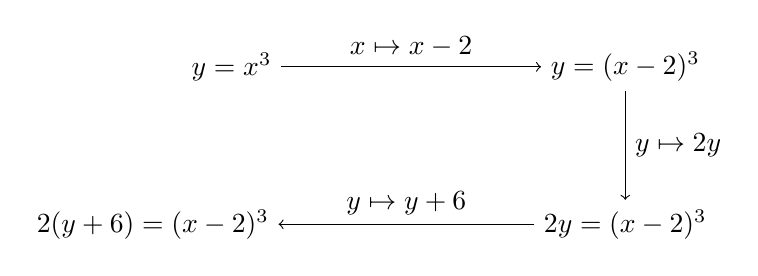
\begin{tikzpicture}
            \node (F) {$y = x^3$};
            \node[right of=F, xshift=4cm] (A) {$y = (x-2)^3$};
            \node[below of=A, yshift=-1cm] (B) {$2y = (x-2)^3$};
            \node[left of=B, xshift=-5cm] (C) {$2(y+6) = (x-2)^3$};

            \draw[->] (F) -- node[anchor=south] {$x \mapsto x-2$} (A);
            \draw[->] (A) -- node[anchor=west] {$y \mapsto 2y$} (B);
            \draw[->] (B) -- node[anchor=south] {$y \mapsto y+6$} (C);
        \end{tikzpicture}
    \end{center}

    Hence, $y = \frac12 (x-2)^3 - 6$

    When $x=0$, $y = -10$. When $y = 0$, $x = 2 + \sqrt[3]{12}$. Thus, the curve crosses the $x$-axis at $(2 + \sqrt[3]{12}, 0)$ and the $y$-axis at $(0, -10)$.
\end{solution}

\begin{problem}
    Find the values of the constants $A$ and $B$ such that $\frac{x^2-4x}{(x-2)^2} = A + \frac{B}{(x-2)^2}$ for all values of $x$ except $x=2$.

    Hence, state a sequence of transformations by which the graph of $y = \frac{x^2-4x}{(x-2)^2}$ may be obtained from the graph of $y = \frac1{x^2}$.
\end{problem}
\begin{solution}
    \[\frac{x^2-4x}{(x-2)^2} = \frac{(x-2)^2 - 4}{(x-2)^2} = 1 + \frac{- 4}{(x-2)^2}.\] Thus, $A = 1$ and $B = -4$.

    \begin{center}\tikzsetnextfilename{246}
        \begin{tikzpicture}
            \node (F) {$y = \dfrac1{x^2}$};
            \node[right of=F, xshift=3.5cm] (A) {$y = \dfrac1{(x-2)^2}$};
            \node[right of=A, xshift=3.5cm] (B) {$y = \dfrac{4}{(x-2)^2}$};
            \node[below of=B, yshift=-1cm] (C) {$y = \dfrac{-4}{(x-2)^2}$};
            \node[left of=C, xshift=-4cm] (D) {$y = 1 + \dfrac{-4}{(x-2)^2}$};

            \draw[->] (F) -- node[anchor=south] {$x \mapsto x-2$} (A);
            \draw[->] (A) -- node[anchor=south] {$y \mapsto \frac14 y$} (B);
            \draw[->] (B) -- node[anchor=west] {$y \mapsto -y$} (C);
            \draw[->] (C) -- node[anchor=south] {$y \mapsto y-1$} (D);
        \end{tikzpicture}
    \end{center}

    \renewcommand{\theenumi}{\arabic{enumi}.}%
    \begin{enumerate}
        \item Translate the curve 2 units in the positive $x$-direction.
        \item Stretch the curve with a scale factor of 4 parallel to the $y$-axis.
        \item Reflect the curve about the $x$-axis.
        \item Translate the curve 1 unit in the positive $y$-direction.
    \end{enumerate}
    \renewcommand{\theenumi}{(\alph{enumi})}
\end{solution}

\begin{problem}
    The transformations $A$, $B$, $C$ and $D$ are given as follows:

    \begin{itemize}
        \item $A$: A reflection about the $y$-axis.
        \item $B$: A translation of 2 units in the positive $x$-direction.
        \item $C$: A scaling parallel to the $y$-axis by a factor of 3.
        \item $D$: A translation of 1 unit in the positive $y$-direction.
    \end{itemize}

    A curve undergoes the transformations $A$, $B$, $C$ and $D$ in succession, and the equation of the resulting curve is $y = 3\sqrt{2-x} + 1$. Determine the equation of the curve before the transformations were effected.
\end{problem}
\begin{solution}
    \begin{alignat*}{2}
        &A \colon x \mapsto -x &&\implies A^{-1} \colon x \mapsto -x\\
        &B \colon x \mapsto x-2 &&\implies B^{-1} \colon x \mapsto x+2\\
        &C \colon y \mapsto \frac13 y &&\implies C^{-1} \colon y \mapsto 3y\\
        &D \colon y \mapsto y-1 &&\implies D^{-1} \colon y \mapsto y+1
    \end{alignat*}

    \begin{center}\tikzsetnextfilename{247}
        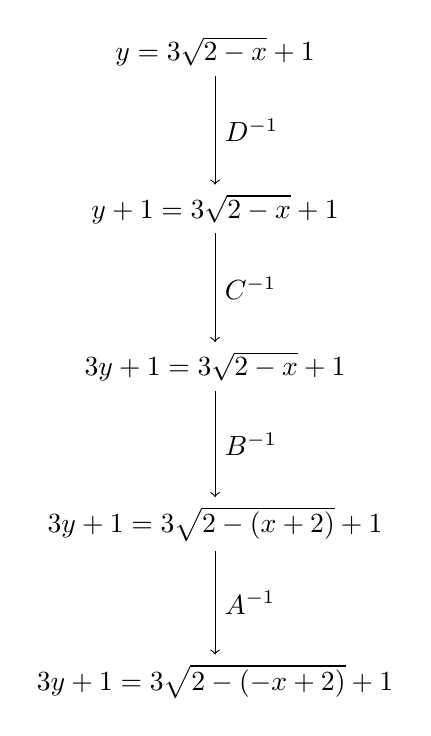
\begin{tikzpicture}
            \node (F) {$y = 3\sqrt{2-x} + 1$};
            \node[below of=F, yshift=-1cm] (D) {$y + 1 = 3\sqrt{2-x} + 1$};
            \node[below of=D, yshift=-1cm] (C) {$3y + 1 = 3\sqrt{2-x} + 1$};
            \node[below of=C, yshift=-1cm] (B) {$3y + 1 = 3\sqrt{2-(x+2)} + 1$};
            \node[below of=B, yshift=-1cm] (A) {$3y + 1 = 3\sqrt{2-(-x+2)} + 1$};

            \draw[->] (F) -- node[anchor=west] {$D^{-1}$} (D);
            \draw[->] (D) -- node[anchor=west] {$C^{-1}$} (C);
            \draw[->] (C) -- node[anchor=west] {$B^{-1}$} (B);
            \draw[->] (B) -- node[anchor=west] {$A^{-1}$} (A);
        \end{tikzpicture}
    \end{center}

    Thus, the original curve has equation $y = \sqrt{x}$.
\end{solution}

\begin{problem}
    \begin{center}\tikzsetnextfilename{248}
        \begin{tikzpicture}[trim axis left, trim axis right]
            \begin{axis}[
                domain=-5:5,
                samples = 101,
                axis y line=middle,
                axis x line=middle,
                xtick = \empty,
                ytick = \empty,
                xlabel = {$x$},
                ylabel = {$y$},
                ymin=-3,
                ymax=5,
                legend cell align={left},
                legend pos=outer north east,
                after end axis/.code={
                    \path (axis cs:0,0) 
                        node [anchor=north east] {$O$};
                    }
                ]
                \addplot[plotRed, domain=-5:0] {2*x * e^(1/2 -1/2 * x^2)};

                \addplot[plotRed, domain=0:2, samples=21, unbounded coords=jump] {3.297 /0.25 * (1/(2-x) - 1/2)};

                \addplot[plotRed, domain=2:5, samples=31, unbounded coords=jump] {1/(x-2) + 2};


                \addlegendentry{$y = f(x)$};

                \fill (-1, -2) circle[radius=2.5 pt];
                
                \node[anchor=north] at (-1.4, -2) {$(-1, -2)$};

                \draw[dotted, thick] (5, 2) -- (-5, 2) node[anchor=south west] {$y=2$};

                \draw[dotted, thick] (2, 5) -- (2, -3) node[anchor=south west] {$x=2$};
            \end{axis}
        \end{tikzpicture}
    \end{center}

    The diagram shows the graph of $y = f(x)$. The curve passes through the origin and has minimum point $(-1,-2)$. The asymptotes are $x=2$, $y=0$ and $y=2$.

    Sketch, on separate diagrams, the graphs of

    \begin{enumerate}
        \item $y = f(x-1)$
        \item $y = f(\abs{x})$
        \item $y = f(\abs{x-1})$
        \item $y = \abs{f(x)}$
        \item $y = \frac{1}{f(x)}$
    \end{enumerate}
\end{problem}
\begin{solution}
    \begin{ppart}
        \begin{center}\tikzsetnextfilename{249}
            \begin{tikzpicture}[trim axis left, trim axis right]
                \begin{axis}[
                    domain=-4:6,
                    samples = 101,
                    axis y line=middle,
                    axis x line=middle,
                    xtick = {-1},
                    ytick = {-2},
                    xlabel = {$x$},
                    ylabel = {$y$},
                    ymin=-3,
                    ymax=5,
                    legend cell align={left},
                    legend pos=outer north east,
                    after end axis/.code={
                        \path (axis cs:0,0) 
                            node [anchor=north east] {$O$};
                        }
                    ]
                    \addplot[plotRed, domain=-4:1] {2*(x-1) * e^(1/2 -1/2 * (x-1)^2)};

                    \addplot[plotRed, domain=1:3, samples=21, unbounded coords=jump] {3.297 /0.25 * (1/(2-(x-1)) - 1/2};

                    \addplot[plotRed, domain=3:6, samples=31, unbounded coords=jump] {1/((x-1)-2) + 2};


                    \addlegendentry{$y = f(x-1)$};

                    \draw[dotted, thick] (6, 2) -- (-4, 2) node[anchor=south west] {$y=2$};

                    \draw[dotted, thick] (3, 5) -- (3, -3) node[anchor=south west] {$x=3$};
                \end{axis}
            \end{tikzpicture}
        \end{center}
    \end{ppart}
    \begin{ppart}
        \begin{center}\tikzsetnextfilename{250}
            \begin{tikzpicture}[trim axis left, trim axis right]
                \begin{axis}[
                    domain=-5:5,
                    samples = 101,
                    axis y line=middle,
                    axis x line=middle,
                    xtick = \empty,
                    ytick = \empty,
                    xlabel = {$x$},
                    ylabel = {$y$},
                    ymin=-3,
                    ymax=5,
                    legend cell align={left},
                    legend pos=outer north east,
                    after end axis/.code={
                        \path (axis cs:0,0) 
                            node [anchor=north east] {$O$};
                        }
                    ]

                    \addplot[plotRed, domain=-2:2, samples=21, unbounded coords=jump] {3.297 /0.25 * (1/(2-abs(x)) - 1/2};

                    \addplot[plotRed, domain=2:5, samples=31, unbounded coords=jump] {1/(x-2) + 2};

                    \addplot[plotRed, domain=-5:-2, samples=31, unbounded coords=jump] {1/(-x-2) + 2};


                    \addlegendentry{$y = f(\abs{x})$};
                    
                    \draw[dotted, thick] (5, 2) -- (-5, 2) node[anchor=north west] {$y=2$};

                    \draw[dotted, thick] (2, 5) -- (2, -3) node[anchor=south west] {$x=2$};

                    \draw[dotted, thick] (-2, 5) -- (-2, -3) node[anchor=south east] {$x=-2$};
                \end{axis}
            \end{tikzpicture}
        \end{center}
    \end{ppart}
    \begin{ppart}
        \begin{center}\tikzsetnextfilename{251}
            \begin{tikzpicture}[trim axis left, trim axis right]
                \begin{axis}[
                    domain=-4:6,
                    samples = 101,
                    axis y line=middle,
                    axis x line=middle,
                    xtick = {1, -1},
                    ytick = {-2},
                    xlabel = {$x$},
                    ylabel = {$y$},
                    ymin=-3,
                    ymax=5,
                    legend cell align={left},
                    legend pos=outer north east,
                    after end axis/.code={
                        \path (axis cs:0,0) 
                            node [anchor=south east] {$O$};
                        }
                    ]
                    \addplot[plotRed, domain=0:1] {2*(x-1) * e^(1/2 -1/2 * (x-1)^2)};

                    \addplot[plotRed, domain=-1:0] {2 * (abs(x)-1) * e^(1/2 -1/2 * (abs(x)-1)^2)};

                    \addplot[plotRed, domain=1:3, samples=21, unbounded coords=jump] {3.297 /0.25 * (1/(2-(x-1)) - 1/2};

                    \addplot[plotRed, domain=-3:-1, samples=21, unbounded coords=jump] {3.297 /0.25 * (1/(2-(abs(x)-1)) - 1/2};

                    \addplot[plotRed, domain=3:6, samples=31, unbounded coords=jump] {1/((x-1)-2) + 2};

                    \addplot[plotRed, domain=-6:-3, samples=31, unbounded coords=jump] {1/((abs(x)-1)-2) + 2};

                    \addlegendentry{$y = f(\abs{x-1})$};

                    \draw[dotted, thick] (6, 2) -- (-6, 2) node[anchor=north west] {$y=2$};

                    \draw[dotted, thick] (3, 5) -- (3, -3) node[anchor=south west] {$x=3$};

                    \draw[dotted, thick] (-3, 5) -- (-3, -3) node[anchor=south east] {$x=-3$};
                \end{axis}
            \end{tikzpicture}
        \end{center}
    \end{ppart}
    \begin{ppart}
        \begin{center}\tikzsetnextfilename{252}
            \begin{tikzpicture}[trim axis left, trim axis right]
                \begin{axis}[
                    domain=-5:5,
                    samples = 101,
                    axis y line=middle,
                    axis x line=middle,
                    xtick = \empty,
                    ytick = \empty,
                    xlabel = {$x$},
                    ylabel = {$y$},
                    ymin=-3,
                    ymax=5,
                    legend cell align={left},
                    legend pos=outer north east,
                    after end axis/.code={
                        \path (axis cs:0,0) 
                            node [anchor=north east] {$O$};
                        }
                    ]
                    \addplot[plotRed, domain=-5:0] {abs(2*x * e^(1/2 -1/2 * x^2))};

                    \addplot[plotRed, domain=0:2, samples=21, unbounded coords=jump] {3.297 /0.25 * (1/(2-x) - 1/2)};

                    \addplot[plotRed, domain=2:5, samples=31, unbounded coords=jump] {abs(1/(x-2) + 2)};


                    \addlegendentry{$y = \abs{f(x)}$};

                    \fill (-1, 2) circle[radius=2.5 pt];
                    
                    \node[anchor=south] at (-1.4, 2) {$(-1, 2)$};

                    \draw[dotted, thick] (5, 2) -- (-5, 2) node[anchor=south west] {$y=2$};

                    \draw[dotted, thick] (2, 5) -- (2, -3) node[anchor=south west] {$x=2$};
                \end{axis}
            \end{tikzpicture}
        \end{center}
    \end{ppart}
    \begin{ppart}
        \begin{center}\tikzsetnextfilename{253}
            \begin{tikzpicture}[trim axis left, trim axis right]
                \begin{axis}[
                    domain=-5:5,
                    samples = 101,
                    axis y line=middle,
                    axis x line=middle,
                    xtick = {2},
                    ytick = \empty,
                    xlabel = {$x$},
                    ylabel = {$y$},
                    ymin=-5,
                    legend cell align={left},
                    legend pos=outer north east,
                    after end axis/.code={
                        \path (axis cs:0,0) 
                            node [anchor=north east] {$O$};
                        }
                    ]
                    \addplot[plotRed, domain=-3:0, samples=61, unbounded coords=jump] {1/(2*x * e^(1/2 -1/2 * x^2))};

                    \addplot[plotRed, domain=0:2, samples=21, unbounded coords=jump] {1/(3.297 /0.25 * (1/(2-x) - 1/2))};

                    \addplot[plotRed, domain=2:5, samples=31, unbounded coords=jump] {1/(1/(x-2) + 2)};


                    \addlegendentry{$y = 1/f(x)$};

                    \fill (-1, -1/2) circle[radius=2.5 pt];
                    
                    \node[anchor=north, fill=white, opacity = 0.6, text opacity=1] at (-1.4, -1/2) {$(-1, -\frac12)$};

                    \draw[dotted, thick] (-5, 1/2) -- (5, 1/2) node[anchor=south east] {$y=\frac12$};
                \end{axis}
            \end{tikzpicture}
        \end{center}
    \end{ppart}
\end{solution}

\begin{problem}
    \begin{center}\tikzsetnextfilename{254}
        \begin{tikzpicture}[trim axis left, trim axis right]
            \begin{axis}[
                domain=-3:3,
                samples=61,
                axis y line=middle,
                axis x line=middle,
                xtick = \empty,
                ytick = \empty,
                xlabel = {$x$},
                ylabel = {$y$},
                legend cell align={left},
                legend pos=outer north east,
                after end axis/.code={
                    \path (axis cs:0,0) 
                        node [anchor=north east] {$O$};
                    }
                ]

                \addplot[plotRed, unbounded coords=jump] {x + 1 + 1/x};

                \addlegendentry{$y=f(a-x)$};

                \addplot[dotted, thick] {x+1};

                \node[rotate=11] at (2, 2.3) {$y = bx+c$}; 

                \fill (1, 3) circle[radius=2.5pt] node[anchor=south] {$(d, e)$};

                \fill (-1, -1) circle[radius=2.5pt] node[anchor=north] {$(f, g)$};
            \end{axis}
        \end{tikzpicture}
    \end{center}

    The graph of $y = f(a-x)$ is shown in the figure, where $a > 0$. The curve has asymptotes $x = 0$, $y = bx+c$, a minimum point at $(d, e)$ and a maximum point at $(f, g)$.

    Given $a > d$, sketch separately, the graphs of 

    \begin{enumerate}
        \item $y = f(x)$
        \item $y = f(\abs{x})$
        \item $y = \frac{1}{f(x)}$
    \end{enumerate}
\end{problem}
\begin{solution}
    \begin{ppart}
        \begin{center}\tikzsetnextfilename{255}
            \begin{tikzpicture}[trim axis left, trim axis right]
                \begin{axis}[
                    domain=-7:9,
                    samples=321,
                    axis y line=middle,
                    axis x line=middle,
                    xtick = \empty,
                    ytick = \empty,
                    xlabel = {$x$},
                    ylabel = {$y$},
                    ymax=20,
                    ymin=-20,
                    legend cell align={left},
                    legend pos=outer north east,
                    after end axis/.code={
                        \path (axis cs:0,0) 
                            node [anchor=north east] {$O$};
                        }
                    ]

                    \addplot[plotRed, unbounded coords=jump] {3 - x + 1/(2-x)};

                    \addlegendentry{$y=f(x)$};

                    \addplot[dotted, thick] {3-x};

                    \draw[dotted, thick] (2, -20) -- (2, 20) node[anchor=north west] {$x = a$};

                    \fill (1, 3) circle[radius=2.5pt] node[anchor=south west, fill=white, opacity = 0.6, text opacity=1] {$(a-d, e)$};

                    \fill (3, -1) circle[radius=2.5pt];
                    
                    \node[anchor=north, fill=white, opacity = 0.6, text opacity=1] at (4, -1) {$(a-f, g)$};
                \end{axis}
            \end{tikzpicture}
        \end{center}

        Equation of asymptote: $y = b(a-x) + c$
    \end{ppart}
    \begin{ppart}
        \begin{center}\tikzsetnextfilename{256}
            \begin{tikzpicture}[trim axis left, trim axis right]
                \begin{axis}[
                    domain=-8:8,
                    samples=321,
                    axis y line=middle,
                    axis x line=middle,
                    xtick = \empty,
                    ytick = \empty,
                    xlabel = {$x$},
                    ylabel = {$y$},
                    legend cell align={left},
                    legend pos=outer north east,
                    after end axis/.code={
                        \path (axis cs:0,0) 
                            node [anchor=north east] {$O$};
                        }
                    ]

                    \addplot[plotRed, unbounded coords=jump] {3 - abs(x) + 1/(2-abs(x))};

                    \addlegendentry{$y=f(\abs{x})$};

                    \addplot[dotted, thick] {3-abs(x)};

                    \draw[dotted, thick] (2, -20) -- (2, 20) node[anchor=north west] {$x = a$};

                    \draw[dotted, thick] (-2, -20) -- (-2, 20) node[anchor=north east] {$x = -a$};

                    \fill (-1, 3) circle[radius=2.5pt] node[anchor=south east, fill=white, opacity = 0.6, text opacity=1] {$(d-a, e)$};

                    \fill (1, 3) circle[radius=2.5pt] node[anchor=south west, fill=white, opacity = 0.6, text opacity=1] {$(a-d, e)$};

                    \fill (-3, -1) circle[radius=2.5pt];
                    
                    \node[anchor=north, fill=white, opacity = 0.6, text opacity=1] at (-4, -1) {$(f-a, g)$};

                    \fill (3, -1) circle[radius=2.5pt];
                    
                    \node[anchor=north, fill=white, opacity = 0.6, text opacity=1] at (4, -1) {$(a-f, g)$};
                \end{axis}
            \end{tikzpicture}
        \end{center}

        Equation of asymptotes: $y = b(a+x) + c$, $y = b(a-x) + c$
    \end{ppart}
    \begin{ppart}
        \begin{center}\tikzsetnextfilename{257}
            \begin{tikzpicture}[trim axis left, trim axis right]
                \begin{axis}[
                    domain=-7:9,
                    samples=321,
                    axis y line=middle,
                    axis x line=middle,
                    xtick = {2},
                    xticklabels = {$a$},
                    ytick = \empty,
                    xlabel = {$x$},
                    ylabel = {$y$},
                    ymin=-1.66,
                    ymax=1,
                    legend cell align={left},
                    legend pos=outer north east,
                    after end axis/.code={
                        \path (axis cs:0,0) 
                            node [anchor=north east] {$O$};
                        }
                    ]

                    \addplot[plotRed, unbounded coords=jump] {1/(3- x + 1/(2-x))};

                    \addlegendentry{$y=\frac1{f(x)}$};

                    \fill (1, 1/3) circle[radius=2.5pt] node[anchor=west] {$(a-d, \frac1{e})$};

                    \fill (3, -1) circle[radius=2.5pt] node[anchor=west] {$(a-f, \frac1{g})$};
                \end{axis}
            \end{tikzpicture}
        \end{center}
    \end{ppart}
\end{solution}

\clearpage
\begin{problem}
    A curve $C_1$ is defined by the parametric equations \[x = t(t+2), \, y = 2(t+1).\]

    \begin{enumerate}
        \item Find the axial intercepts of the curve.
        \item Sketch $C_1$.
        \item A curve $C_2$ is defined by the parametric equations $x = t(t+2), \, y = t+1$. Describe a geometrical transformation which maps $C_1$ to $C_2$. Hence, sketch the curve $C_2$ in the same diagram as $C_1$.
        \item Show that the Cartesian equation of the curve $C_1$ is given by $y^2 = 4(x+1)$.
    \end{enumerate}
\end{problem}
\begin{solution}
    \begin{ppart}
        Consider $x = 0$. Then $t(t+2) = 0$, whence $t = 0$ or $t = -2$. When $t = 0$, $y = 2$. When $t = -2$, $y = -2$. Hence, the curve intercepts the $y$-axis at $(0, 2)$ and $(0, -2)$.

        Consider $y = 0$. Then $t = -1$, whence $x = -1$. Hence, the curve intercepts the $x$-axis at $(-1, 0)$.
    \end{ppart}
    \begin{ppart}
        \begin{center}\tikzsetnextfilename{258}
            \begin{tikzpicture}[trim axis left, trim axis right]
                \begin{axis}[
                    xmin=-2,
                    axis y line=middle,
                    axis x line=middle,
                    xtick = {-1},
                    ytick = {2, -2, 1, -1},
                    xlabel = {$x$},
                    ylabel = {$y$},
                    legend cell align={left},
                    legend pos=outer north east,
                    after end axis/.code={
                        \path (axis cs:0,0) 
                            node [anchor=north west] {$O$};
                        }
                    ]

                    \addplot[plotRed] [domain=-3:1,samples=100]({x * (x+2)},{2 * (x + 1)});

                    \addlegendentry{$C_1$};

                    \addplot[plotBlue] [domain=-3:1,samples=100]({x * (x+2)},{(x + 1)});

                    \addlegendentry{$C_2$};
                \end{axis}
            \end{tikzpicture}
        \end{center}
    \end{ppart}
    \begin{ppart}
        Scale by a factor of $\frac12$ parallel to the $y$-axis.
    \end{ppart}
    \begin{ppart}
        \[y^2 = (2(t+1))^2 = 4(t^2 + 2t + 1) = 4(t(t+1) + 1) = 4(x + 1).\]
    \end{ppart}
\end{solution}